\documentclass{article}

\usepackage{minted}
\usepackage{amsmath, amsthm}
\usepackage{listings}
\usepackage[svgnames]{xcolor}
\usepackage{tikz}
\usepackage{array}
\usepackage{graphicx}
\usepackage{biblatex}

\usemintedstyle{solarized-light}
\setminted{fontsize=\footnotesize, bgcolor=Beige}

% NOTE: need to run `biber adt_survey` to ensure up-to-date references
\addbibresource{adt_survey.bib}

\title{A Survey on Abstract Data Types}
\author{Anthony Hunt}

\begin{document}
\maketitle

\section{Introduction}

From the categorization of species to the periodic table of elements, the organization and manipulation
of data is integral to all aspects of science and technology. Although the collection of data is not a
new field of research by any means, the advent of computerized systems, with its ability to transfer and use
massive amounts of data in mere seconds, necessitates understandable and sensible organization structures.

Over the past 60 years, as computational resource restrictions have eased dramatically,
programming languages and software creation tools have evolved with increasingly better methods of dealing with data.
By viewing pieces of data through specific lenses, programmers can then write algorithms that operate on
any data matching the shape of those lenses, rather than the data itself. These lenses are more commonly referred to as
data types, which assign a type to a piece of data. As we will see later in this paper,
further abstractions over data types themselves enable extremely concise and readable code,
both for the programmer and computer.

The rest of this article will explore data type concepts from <X> languages, % TODO FILL IN
structures to handle errors that might appear, and a small review of ergonomics and usability of those data types.
A necessary discussion of various type systems will naturally evolve as a precursor to data types themselves.

\section{Data Types in <X>+ Languages} % TODO fill in value for X!!!!!!!!!!!!!!!!!!!!!!!!!!!!!!!!!!!!!!!

Abstract Data Types (ADTs) can look quite different in many languages, but often share the same principles and rules
that make it understandable for programmers. In its essential form, an ADT is a collection of data together with
operations that can be carried out on that data \cite{ADTspec}. The key differences between ADTs from different languages
are the conventions used to collect data and the power operations have over collected data.

In popular object-oriented programming (OOP) languages,
ADTs are approached with a ``class'' mindset, where programmers specify a blueprint for objects that
will eventually be used in a program. For better code reuse, classes can be built from pre-existing classes
through the use of inheritance, a term used to express that a new class inherits all the properties of the old class.
Objects created by classes are referred to as instances of the class and often hold
some amount of mutable data, with methods that have full access to the data. The methods can choose to make use of
``side effects'', referring to the modification of data not explicitly passed through
regular function arguments or return values. Side effects in methods have the consequence that the output of
a method may change independent of the values passed through its arguments. In other words,
the object a method has access to may contain some state that influences the outcome of the method.

At the opposite end of the programming world lies purely functional languages. ADTs in these languages
are more often referred to as data types rather than classes and are only used for collecting and operating on data.
``Objects'' created from these data types are immutable and methods are instead replaced with pure functions that
explicitly take in the relevant data type as input. The operators attached to a functionally pure ADT are functionally
pure themselves, meaning they cannot make use of any hidden state and therefore cannot have side effects.

% Type to express in all languages - a simple linked list, with append and concatenate methods
\subsection{Python}

As a dynamic interpreted scripting language with thousands of high quality libraries and a short learning curve,
Python has become one of the most dominant modern programming languages across several subdomains of computing.
The language itself is characterized mainly by its simple approach to writing readable, practical, and user-friendly code \cite{pythonZen},
used by many as a ``glue'' to easily join high performance computing libraries. The role of Python as a mediator
between optimized C libraries and human understanding, especially in the machine learning space, is adjacent to the role
of documentation in expressing the intention and meaning behind code,
rather than focusing on the small details of the code itself.
% early-age low-level languages and hand-optimized assembly. The abstractions provided from assembly to C,
% and now C to Python, are evident of the trend towards using higher level languages for a better developer experience.
% TODO refer to above comment in the rust section instead

\subsubsection{Python and Types}

The overarching data model behind Python is that everything is either an object or a relation between objects.
Almost all objects in Python are used by reference, and each object contains an identifier (memory address),
an immutable type, and then the actual value itself. In contrast to other scripting languages (namely JavaScript),
an immutable type means that Python will never implicitly recast the type of an object to fit the expected types
of functions or methods (ie. it is strongly typed).

% This behaviour is very different to types in static languages, where names are assigned a type at compile time;
% the runtime objects know their own type and determine which operations can be performed. Thankfully, because of strong
% typing,

Although Python is strongly typed, its lack of a static typing system serves as a double edged sword for
readability and reliability. With small programs, some developers may prefer to just ``get things done'',
making use of whatever combination of builtin types are available.
A mixture of sets, dictionaries, and lists with unrestricted element types are all too common in these types of scripts.
However, assigning proper data types to work with various pieces of information is essential
to the longevity and maintenance of large scale projects. Since the introduction of optional static type hints
via a library in Python 3.5 and increased support through Python 3.8,
a 2022 survey \cite{empiricalTypePython} found a steady increase in the number of GitHub repositories
making use of static type hints.

Aside from granting linters more information to statically analyze the program and warn developers of possible errors,
types also provide programmers themselves with useful information regarding their program. As reinforced
by the philosophy of TypeScript as a type-hinted version of JavaScript, data types serve as an important
channel of communication between programmers. An additional finding of the 2022 survey \cite{empiricalTypePython}
showed that typecheck errors in the linters did not prevent a large amount of code from being pushed, but were
still found to be useful outside of the linter.

Fundamentally, Python places little restriction on the programmer's actions. For example, while
data privacy within Python objects is theoretically possible through name mangled fields (beginning with double-underscores),
there is no real way to completely restrict access to an object's fields so long as that object exists in the code.
Access to deeper implementation details, like a list of current variables, list of fields in any variable, and even
interpreted bytecode is possible through the use of magic methods and variables
(denoted by two underscores at the beginning and end of the identifier).

\subsubsection{Example: A Linked List}

Since Python is primarily an OOP language, the most common form of expressing data types is through the use of classes.
A typical linked list data type in Python 3.11 would look something like:
\inputminted{python}{linked_list/main.py}

Note that Python 3.12 and later make some major changes involving scoping and the syntax of generic types \cite{pythonGenericTypeChange}.

The above \texttt{LinkedList} class expresses the recursive linking nature of the data type while demonstrating
commonly used side effects of OOP methods. Note that the return type for both \texttt{append} and \texttt{concat}
is \texttt{None}. Instead, the data contained within the \texttt{self} object is mutated in place as needed to achieve
the desired functionality.

\subsubsection{Pydantic: A data validation library}

While native Python works well for simple data types like linked lists, type hints do not provide any guarantees
that the type of value, for example, will be consistent across all elements in the list. So, while it does serve as a useful
notation tool for documenting the structure of a data type to other programmers, there are no insurance that the runtime
values for these objects are consistent with the type annotations. As with many topics in Python, a convenient library by the name
of Pydantic will enable both type hints and data validation for those types \textit{at runtime}. The Pydantic version
of our linked list will now look something like:
\inputminted{python}{linked_list/main_pydantic.py}

For this simple data type, only the init function changes. However, under the hood, Pydantic will now ensure that
the type of \texttt{value} within this linked list remains consistent across all elements, throwing an exception
otherwise. Pydantic's version of a class has the ability to transform an OOP construct into one more closely related
to functional programming. If desired, the use of decorators above field names or methods (denoted by \texttt{@decorator})
can restrict mutability, modify constructors, and even change the data validation process to ensure objects are of the correct type.

\subsubsection{Conclusion}

Python's high-level nature, excellent documentation, library support, and exposure of underlying architectures when needed
combine to create a powerful, flexible, and productive language. Although many aspects of the language are initially
hidden or abstracted for the sake of convenience, Python allows programmers to dig deeper into the implementation
when necessary and extend the language in a manner best suited for a specific task.

\subsection{TypeScript}

In JavaScript, types are very loosely bound, and many operations/functions will silently convert types
at runtime. The silent recasting of JavaScript objects combined with unintuitive defaults
can result in very confusing results for the uninitiated. For example, the expression \texttt{1 + "1"}
returns a value of 11 and the expression \texttt{[5, 11, 2].sort()} returns
\texttt{[11, 2, 5]}. In both expressions, the numerical values are converted into strings before the operation is performed.

TypeScript, as an extension of JavaScript with types, is similar to Python in the sense that both
languages started with dynamic typing and patched on static types after the fact, and both aim to resolve issues caused
by dynamic typing. TypeScript (and Python) use types not only for more assurance in program correctness,
but also for the sake of convenience. When making full use of the available typing systems, text editors
and IDEs are able to assist in new code development through intellisense and autocompletion of methods and variables.
Types of objects and documentation for those types additionally appear on mouse-hover, providing fast in-context knowledge.

The below list outlines key properties of types in TypeScript.
\begin{itemize}
    \item Types are treated as sets of values, where types can be part of multiple sets,
    a union of sets, or rarely even an intersection of sets.
    \item Types are structural. Any object containing the required fields needed to be a member of a certain type
    will be considered an object of that type, even if a different type name has been assigned to it.
    Further, if an object has additional fields not specified by the type,
    the extra fields will be ignored in the typechecking process. Essentially, as long as an object meets the minimum
    fields required by the specified type, the object is assumed to be a member of that type.
    \item TypeScript allows any literal string to act as a subset of its respective type,
    with the only allowed value being the literal itself.
    For example, a field with the type \texttt{``name''} will only accept the value of ``name''.
    However, a field with the type \texttt{String} will accept any string object.

\end{itemize}

In comparison to algebraic data types often seen in functional languages, TypeScript replaces inductive data types
with discriminated union sets. For example, our linked list type may look something like:
\inputminted{typescript}{linked_list/main.ts}

Because TypeScript allows literals to act as types, the only valid values in the ``kind'' field
of an object represented by the \texttt{LinkedList} type are our constructor names: ``nil'' or ``cons''.
Although TypeScript treats every object as a reference, similar to Python, we have not used side effects
in the \texttt{append} or \texttt{concat} functions. Instead, we explicitly accept the linked list we want to transform as
input, perform the required action, and return the head of the linked list in the output.

For a non-inductive approach to the LinkedList data type, we can use TypeScript's interfaces to create something that
looks much more like the Pydantic version:
\inputminted{typescript}{linked_list/main_interface.ts}

Finally, a pure OOP version of our LinkedList type, using classes, can be formed.
Note that the append and concat functions are now methods with side effects:
\inputminted{typescript}{linked_list/main_class.ts}

% \subsection{C++}
\subsection{Rust}
\subsection{Dafny}
\subsection{Haskell}
\subsection{Agda}
\subsection{APL}

\subsection{Unified Modelling Language (UML)}

Up until this point, all the languages explored in this document have been targeted at making computers
execute a desired set of instructions over some type of data. Of course, the specific methodology
and concepts used to achieve this human-computer interaction differ greatly between languages,
with each maintaining their own idioms and customs. Conversely, UML is not a programming language in
the normal sense, but a standardized method of visualizing and clearly communicating the intentions behind a system.

According to the UML documentation, UML is intentionally independent of any and all processes that could be used
to actually implement a system. UML diagrams are not intended to comprehensively cover every aspect of a system's implementation,
including different quirks and features of different languages, but rather should be used as a powerful aid in
the creation of program documentation. Generally, different types of diagrams are used for recording types, state, information flow,
and even the execution of the program itself.

In the context of UML, a data type is a specialized form of classifier with no internal structure. Each data type may contain
several named fields to contain data, along with operations on that data.
The focus of data type based diagrams is to convey the following to programmers:
\begin{enumerate}
    \item All data types available to the user.
    \item All relationships between data types, including inheritance, extensions, use of types within the fields of other types,
    and even type usage in operators.
\end{enumerate}

Below is an example of our famous LinkedList type, modelled by UML:
\begin{center}
    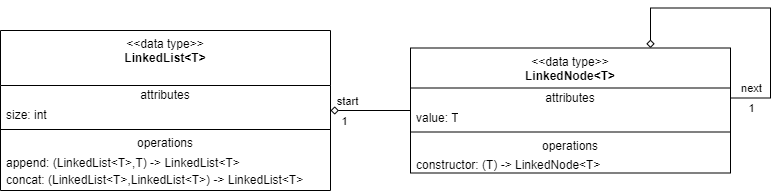
\includegraphics[width=12cm]{linked_list/uml.drawio.png}
\end{center}

A simple standalone type like LinkedList may not be complex enough to showcase the full advantages of UML,
but it is enough to demonstrates the effectiveness of visualization in understanding code.
From the arrows in the image, it is immediately obvious that the start attribute of
LinkedList requires a LinkedNode and LinkedNodes may build off of themselves indefinitely.

UML diagrams are a simple and concise method for conveying the meaning and intention behind a system.
While the syntax is largely standardized, because this language is meant for communication with humans
rather than machines, slight modifications of syntax for the sake of clarity can be made as necessary.
For example, the types of operators may be omitted for an ultra-compact diagram, or kept to ensure an agreement
on the interface implementation is met.

\subsection{Event-B}

Although UML is a powerful tool for communicating the relationship between data types, the visual methodology
falls short when attempting to convey the actionable properties of a system. In continuing the exploration
of modelling languages, we find that the Event-B model not only encompasses actionable system traits, but does
so with consideration of the system's environment. Therefore, Event-B is suitable for formal system analysis
and proving the correctness of software following the model specification.

Data types for Event-B may not exist in the normal sense of the word, but a different approach to data abstraction
through the concepts of machines, contexts, and events is more than suitable for the same purpose:
\begin{itemize}
    \item Machines are somewhat adjacent to classes in OOP, acting like miniature
    programs with some provable traits consisting of variables, invariants, theorems, a single variant, and a list of
    events that may cause the machine to ``run'' (analogous to an object's methods).
    Like class inheritance, new machines can ``refine'' old ones by
    carrying over and adding new entries to the aforementioned traits.
    \item Contexts, on the other hand, are much closer the formal definition of abstract data types,
    defining a set of axioms, theorems, constants and data in the form of carrier sets.
    Contexts can be extended in a similar fashion to class inheritance, with the child context carrying over all properties
    of the parent context.
    \item Finally, events serve as activation conditions for the machine they are assigned to.
    They introduce possibly nondeterministic actions into the system in a formal manner, and must clearly state
    how they affect a machine's variant. A key aspect of events is that all actions within an event are performed simultaneously.
    This means that, unlike in sequential programming languages, the order in which actions are defined have no relevance
    on the outcome of the event. Of course, the restriction of simultaneous execution means that users of the language
    cannot reassign variables in more than one action, nor should they rely on the deterministic nature of normal program execution.
\end{itemize}
All expressions in the above abstractions use formal discrete math notation.

Although a modelling language focused on provable aspects of a system
is not very suitable for a simple low-level data type,
we nonetheless attempt a simplified implementation of \texttt{LinkedList} with only the append method.

\begin{center}
    \fbox{
        \parbox{12cm}{
            LinkedListContext

            \hspace{2em}\textbf{sets}

            \hspace{4em}$Nodes$ // Set of nodes in the list

            \hspace{4em}$References$ // Set of references

            \hspace{2em}\textbf{constants}

            \hspace{4em}$null$ // End of list

            \hspace{2em}\textbf{axioms}

            \hspace{4em}axm1: $References = Nodes \cup \{null\}$

            \hspace{4em}axm2: $\forall n : n \in Nodes \implies n.next \in References$ // All nodes must have a reference

        }
    }
    \fbox{
        \parbox{12cm}{
            AppendEvent

            \hspace{2em}\textbf{any}

            \hspace{4em}$last\_node$

            \hspace{4em}$new\_node$

            \hspace{2em}\textbf{where}

            \hspace{4em}$last\_node \in Nodes$

            \hspace{4em}$\{last\_node\} = \{node \in Nodes : node.next = null \}$ // last\_node is the end of the list

            \hspace{4em}$new\_node.value: T$ // New value must have the same type as existing nodes

            \hspace{4em}$new\_node.next = null$ // New node is end of the list

            \hspace{2em}\textbf{then}

            \hspace{4em}$last\_node.next := new\_node$ // Last node is no longer the last node

            \hspace{4em}$Nodes := Nodes \cup new\_node$ // Add node to list


        }
    }
    \fbox{
        \parbox{12cm}{
            LinkedListMachine

            \hspace{2em}\textbf{variables}

            \hspace{4em}$head$

            \hspace{4em}$value$

            \hspace{4em}$next$

            \hspace{2em}\textbf{invariant}

            \hspace{4em}inv1: $head \in Nodes$

            \hspace{4em}inv2: $value: T$ // Generic type T

            \hspace{4em}inv3: $next \in References$

            \hspace{4em}inv4: $\forall n : n.next \neq null \implies n.next.next \in References$ // Nodes can either end or continue the list

            \hspace{2em}\textbf{events}

            \hspace{4em}AppendEvent

        }
    }
\end{center}

The latest Event-B wiki \cite{eventB} notes future plans to support recursive structured types like inductive LinkedLists
in a more concise format.

% \subsection{SETL} %Maybe? Would need to cite
% \subsection{Bend} %Maybe? Would need to cite
\subsection{Exploration of Conceptual Data Types}

\subsubsection{The Axiomatic Approach to Data Types}

As stated in the introductory textbooks \cite{DTandDS} and \cite{ADTspec}, ADTs at their core are just collections of
data coupled with operations. Both textbooks introduce data types in a manner not unlike the ideas of Event-B,
using formal notation to guarantee precise properties of the given data type. Interestingly, both textbooks
opt to separate data type operations into syntactic and semantic components, where the semantics
contain a list of axioms to be fulfilled by each operation. Note that these axioms are almost entirely removed
from the implementation of the type, acting more as a specification of requirements rather than a how-to guide.

Guaranteed type completeness and correctness are two key features of the axiomatic approach. That is, axioms
encourage operations to consider all possible values that the type may take, especially regarding edge cases and errors.
For example, in our linked list, we need to ensure operations over an empty list are well-defined and that we can
create the empty list itself in the first place. Of course, in the case of linked lists, this is near-trivial,
but focusing on the edge cases in this manner can guarantee correctness of far more complex types.

Consider the axiomatic definition of a linked list, according to the specification of \cite{ADTspec}:
\begin{center}
        \parbox{11cm}{
            NAME

            \hspace{2em}LinkedList(item)

            SETS

            \hspace{2em}$N$: Set of nodes

            \hspace{2em}$I$: Set of items

            SYNTAX

            \hspace{2em}$new: \rightarrow N$

            \hspace{2em}$append: N \times I \rightarrow N$

            \hspace{2em}$concat: N \times N \rightarrow N$

            \hspace{2em}$deleteLast: N \rightarrow N$

            \hspace{2em}$tail: N \rightarrow I$

            \hspace{2em}$isEmpty: N \rightarrow bool$


            SEMANTICS

            $\forall i \in I, \forall n, n1 \in N:$

            \hspace{2em}$deleteLast(append(n, i)) = n$

            \hspace{2em}$tail(append(n, i)) = i$

            \hspace{2em}$tail(concat(n, n1)) = tail(n1)$

            \hspace{2em}$isEmpty(new()) = True$

            \hspace{2em}$isEmpty(append(n, i)) = False$

            \hspace{2em}$tail(new()) = error$ // New initializes a list but does not hold any value

            \hspace{2em}$deleteLast(new()) = error$ // Cannot delete from an empty list

    }
\end{center}

The above axioms do not express the behaviour of each function independently, but instead focus on relationship between one another.
For instance, the axiom $tail(new()) = error$ outlines two properties with one axiom:
\begin{enumerate}
    \item Finding \texttt{tail} on an empty list produces an error.
    \item Since tail produces an empty list error, we must know that \texttt{new} creates an empty list.
\end{enumerate}
Similarly, the axiom $deleteLast(append(n, i)) = n$ shows that append must add the item $i$
to the end of the list $n$, in order for deleteLast to perform correctly.

Unfortunately, this approach may present drawbacks for implementing unknown data types in popular programming languages
\textit{because} of its coupled operation behaviour. In many programming languages, especially non-functional ones,
developers need to implement each data type operation mostly independent of other operations. Therefore, ensuring congruency
between written code and the given specification presents a new challenge for programmers;
data types becoming lost in the translation from dependent specification to independent implementation serve
as an undesirable source of bugs and mistakes. A compiler for such a language would greatly reduce friction between
theory and application, but the semantic expressivity available from the axiomatic approach may be worth the costs.

\subsubsection{A More Constructive Approach}

The textbook \cite{ADTspec} specifies an additional method of data type specification focused on construction
of new objects from old ones. Instead of axioms, each operation can specify relevant pre-conditions and post-conditions.
This method is far closer to the implementation of data types in programming languages, with an uncanny resemblance
to the optional input restrictions seen in Dafny functions. For conciseness, the example given in Section 2.4
serves as a good approximate illustration of the constructive approach outlined in the textbook.

\section{Error Handling and Undefinedness}
\section{A Word on Usability}
\section{Conclusion}


\nocite{*} % keeps all references, even those not referred to
\printbibliography %Prints bibliography

\end{document}